\documentclass[preprint,12pt,authoryear]{elsarticle}
\usepackage[T1]{fontenc}
\usepackage[utf8]{inputenc}
\usepackage{amsmath,amssymb}
\usepackage{graphicx}
\usepackage{booktabs}
\usepackage{multirow}
\usepackage{algorithm}
\usepackage[noend]{algpseudocode}
\usepackage{textcomp}
\usepackage{gensymb}
\usepackage[hidelinks]{hyperref}
\usepackage{lineno}
\linenumbers
\biboptions{authoryear}

\journal{Artificial Intelligence in Agriculture}

\begin{document}

\begin{frontmatter}

\title{Learning to share sunlight: differentiable-simulation design and control of climate-resilient agrivoltaics across the world's staple croplands}

\author{Quang-Vinh Dang\corref{cor1}}
\ead{vinh.dq4@buv.edu.vn}
\cortext[cor1]{Corresponding author.}
\address{British University Vietnam, Hung Yen, Vietnam}

\begin{abstract}
Solar power and food production increasingly compete for the same land, while warming exposes crops to more heat and drought. Agrivoltaic systems, which grow crops under photovoltaic (PV) modules, can relieve this conflict, but how much electricity farmland can produce without compromising food security depends on how sunlight is shared between modules and plants, day by day, for every crop and climate. We propose SALS (stress-aware light sharing), an algorithm that learns the design and the daily control of single-axis tracker agrivoltaics end-to-end through a differentiable simulator. The simulator couples solar geometry, backtracking trackers, PV output, crop-level light and microclimate, a soil-water balance and the SIMPLE crop model with heat and drought stress. A design network maps site descriptors to the ground coverage ratio, and a control network maps the daily crop, soil and weather state to the tracker's light-sharing level. Both are trained by back-propagation through whole seasons to maximise electricity subject to a 90\% yield-retention floor. We applied SALS to 400 sites representing the global harvested area of wheat, rice, maize, soybean and potato, with NASA POWER weather for 2001--2019 and warming of +1.5, +2 and +3\,\textdegree C. On geographically held-out sites and years, SALS produced 1019\,MWh\,ha$^{-1}$\,yr$^{-1}$ (72\% of a conventional PV plant) at a mean yield retention of 0.91. This gave a land-equivalent ratio of 1.63, compared with 1.20 for static agrivoltaic designs and 1.42 for an expert stress rule ($p<10^{-4}$). Its advantage grew with warming, to an LER of 1.75 at +3\,\textdegree C, as the learned policy shifted from sharing light during canopy development to shading crops during heat. The yield floor was met on average but in only 45--49\% of individual seasons, which calls for chance-constrained extensions. Scaled to 5\% of the harvested area of the five crops, learned agrivoltaics has a technical potential of about 31{,}000\,TWh\,yr$^{-1}$, comparable to current global electricity generation.
\end{abstract}

\begin{keyword}
Agrivoltaics \sep Differentiable simulation \sep Food--energy nexus \sep Climate adaptation \sep Solar tracking \sep Crop modelling \sep Physics-informed machine learning
\end{keyword}


\end{frontmatter}

\section{Introduction}\label{sec:intro}

Two of the defining challenges of this century compete for the same resource: land. The energy transition requires terawatts of new solar photovoltaic (PV) capacity, and ground-mounted solar farms need roughly one to two hectares per megawatt. Food production must rise while crops are exposed to more frequent heat waves and droughts. Warming alone is projected to reduce global yields of maize, wheat, rice and soybean by several per cent per degree \citep{zhao2017}, and a new generation of climate and crop models shows these impacts emerging earlier than previously expected \citep{jagermeyr2021}. Croplands are also where solar power potential is greatest \citep{adeh2019}. They are flat, sunny, accessible and close to rural electricity demand, so converting farmland into solar farms is tempting and controversial at the same time.

Agrivoltaic (AV) systems combine crops and PV modules on the same land and aim to resolve this conflict \citep{dupraz2011,dinesh2016,weselek2019}. By sharing sunlight between modules and plants, a hectare can deliver more food plus energy than the two uses side by side, with land-equivalent ratios (LER) well above one in field trials and modelling studies \citep{dupraz2011,amaducci2018,valle2017,trommsdorff2021}. The partial shade also changes the crop microclimate. It lowers canopy temperature and evaporative demand, conserves soil moisture and improves water-use efficiency, especially in drylands \citep{marrou2013,adeh2018,barron2019,elamri2018,weselek2021}. Agrivoltaics is therefore a candidate adaptation measure against heat and drought stress, in addition to a mitigation measure through renewable electricity. The same shade, however, also reduces the light available for photosynthesis. Regulators increasingly require AV systems to retain most of the reference crop yield. The German pre-standard DIN SPEC 91434, for example, requires at least 66\% of the reference yield \citep{din2021}, and other schemes and many farmers set stricter floors. How much electricity can be produced without sacrificing food security depends on the crop, the local climate, the year and the growth stage.

Most AV designs fix the geometry of the array, i.e.\ the ground coverage ratio (GCR, module area per ground area) and the tilt or tracking rule, from generic rules of thumb. Single-axis trackers add a degree of freedom: the modules can be rotated away from the sun to let light through when the crop needs it, as demonstrated for lettuce by \citet{valle2017}, or towards the sun to maximise electricity and shade the crop during heat waves. Choosing the rotation every day is a sequential decision problem. The value of light depends on the crop's phenological stage, soil water and upcoming weather, and the effect of a decision appears in the harvest months later. Designing the GCR and the control policy for every combination of crop and climate on Earth, and for a warming climate, is beyond manual rule design. Recent work in this journal has used evolutionary multi-objective optimisation to lay out PV arrays on farmland \citep{zhang2026}. Machine learning for crop management has mainly used reinforcement learning with black-box simulators \citep{gautron2022}, which is sample-inefficient and hard to scale to global, multi-decadal assessments.

This paper proposes \emph{SALS} (stress-aware light sharing), a learning algorithm that designs and controls agrivoltaic systems jointly, for any cropland site on Earth, through a differentiable physics simulator. The simulator couples hourly solar geometry, single-axis trackers with backtracking, row-to-row shading and PV electricity, the direct and diffuse light reaching the crop, a microclimate model of canopy temperature and reference evapotranspiration under the modules, and the SIMPLE crop model with heat and drought stress \citep{zhao2019}. Because every component is written as differentiable tensor operations, two small neural networks can be trained by gradient descent through entire growing seasons. A \emph{design network} maps site descriptors to the GCR, and a \emph{control network} maps the daily crop and soil state and the same-day weather forecast to the tracker's light-sharing level. Training maximises electricity subject to a yield-retention floor, across hundreds of sites, twenty years of weather and four warming levels. This physics-informed learning approach \citep{karniadakis2021} gives a single policy that generalises to unseen regions, years and climates.

We apply SALS to 400 sites that represent where maize, wheat, rice, soybean and potato are grown worldwide, sampled in proportion to their harvested area \citep{yu2020} with local crop calendars \citep{jagermeyr2021}, and driven by NASA POWER daily weather for 2001--2019 \citep{sparks2018}. The contributions are as follows.
\begin{enumerate}
\item A differentiable agrivoltaic simulator that couples tracker geometry, PV output, crop-level light and microclimate, soil water and a generic crop model, and runs thousands of site-seasons in parallel on a CPU.
\item The SALS algorithm, which learns the array design and a closed-loop, stress-aware tracker policy end-to-end under a food-security constraint. It is evaluated on geographically held-out sites and years against static designs, expert rules and a perfect-foresight oracle.
\item A global assessment under warming of +1.5, +2 and +3\,\textdegree C, which quantifies how much electricity croplands can supply while retaining at least 90\% of crop yields, and where agrivoltaics protects yields against heat and drought.
\end{enumerate}

\section{Materials and methods}\label{sec:methods}

\subsection{Global cropland sites, weather and crop calendars}\label{sec:data}
We studied five staple crops that together cover about 670\,Mha of harvested area: wheat, rice, maize, soybean and potato. Harvested areas (rainfed and irrigated) were taken from the SPAM 2010 gridded production maps \citep{yu2020} and aggregated to 1\textdegree{} cells. For each crop, 80 cells with at least 5000\,ha of the crop were drawn without replacement with probability proportional to harvested area. An unweighted average over the sample therefore approximates an area-weighted average over global production. The 400 crop--site pairs lie in 381 distinct cells in 50 countries (Fig.~\ref{fig:map}). Sowing and maturity dates came from the GGCMI Phase~3 crop calendar at 0.5\textdegree{} \citep{jagermeyr2021}. For wheat we used the winter-wheat calendar unless the coldest-month mean temperature was below $-8$\,\textdegree C, in which case the spring-wheat calendar was used. Daily weather for 2001--2020 was retrieved from NASA POWER \citep{sparks2018}: global and diffuse shortwave irradiance, maximum, minimum and dew-point temperature, precipitation and wind speed at 2\,m. Each site contributes 19 seasons (sowing years 2001--2019), each simulated as the 365 days after sowing, which gives 7600 site-seasons.

Climate change was represented by the global warming levels +1.5, +2 and +3\,\textdegree C relative to 2001--2020. Daily maximum, minimum and dew-point temperatures were shifted uniformly, which keeps relative humidity approximately constant and raises the vapour-pressure deficit. The atmospheric CO$_2$ concentration was set to 390, 450, 500 and 600\,ppm for the baseline and the three warming levels. Precipitation and irradiance were left unchanged. This delta approach isolates the thermal signal of warming; its limitations are discussed in Section~\ref{sec:limits}.

\subsection{A differentiable agrivoltaic simulator}\label{sec:sim}
The simulator advances all site-seasons in parallel with a daily time step for the crop and an hourly time step for radiation and PV (Fig.~\ref{fig:scheme}). All equations are implemented as PyTorch tensor operations \citep{paszke2019}, so that yields and electricity are differentiable with respect to the design and control variables.

\paragraph{Hourly irradiance}
Daily global and diffuse irradiance were disaggregated into hourly values with the \citet{collares1979} and \citet{liu1960} ratios and renormalised to the daily totals. Beam irradiance on the horizontal is the difference between the two. Solar position follows the standard declination and hour-angle equations.

\paragraph{Array geometry and PV electricity}
We consider elevated horizontal single-axis trackers with north--south axes. The axis height is $1.25$ module widths, which leaves space for machinery under the modules. The rotation $\phi$ is limited to $\pm60^\circ$, and the ground coverage ratio $g$ is the module width divided by the row pitch. Let $\psi$ be the solar zenith angle projected onto the east--west vertical plane. The energy-optimal rotation with backtracking \citep{lorenzo2011} is $\phi_{\mathrm{bt}}=\psi-\mathrm{sgn}(\psi)\arccos(\cos\psi/g)$ when $\cos\psi<g$, and $\phi_{\mathrm{bt}}=\psi$ otherwise. The \emph{light-sharing} rotation $\phi_{\mathrm{sh}}$ is the feasible angle closest to edge-on to the sun, which minimises the shadow on the crop. Given a light-sharing level $u\in[0,1]$ chosen once per day, the rotation in every hour is
\begin{equation}
\phi = (1-u)\,\phi_{\mathrm{bt}} + u\,\phi_{\mathrm{sh}}.
\label{eq:phi}
\end{equation}
Plane-of-array irradiance combines beam irradiance on the module (reduced by the fraction of the module shaded by the neighbouring row, $\max\{0,1-\cos\psi/(g\,|\cos(\phi-\psi)|)\}$), isotropic sky diffuse and ground-reflected light (albedo 0.2). The cell temperature follows the NOCT model (45\,\textdegree C), with an hourly air temperature interpolated sinusoidally between the daily extremes. Electricity per unit land is plane-of-array irradiance $\times\,\eta\times g$, with $\eta=0.21\,[1-0.0035(T_{\mathrm{cell}}-25)]\,(1-0.14)$ for module efficiency, temperature losses and system losses. A conventional ground-mounted PV plant ($g=0.4$, backtracking, no crop) is the energy reference $E_{\mathrm{PV}}$.

\paragraph{Light and microclimate at the crop}
Averaged over the row pitch, the fraction of ground reached by beam light is $1-\min\{1,\,g\,|\cos(\phi-\psi)|/\cos\psi\}$. The fraction of sky diffuse reaching the ground is a two-dimensional isotropic sky-view factor. We pre-computed it for 25 values of $g$ and 13 rotation angles by ray casting over 31 neighbouring rows, and interpolate it bilinearly (differentiably). The daily ratio $s$ of the irradiance at the crop to that of the open field defines the crop's shading. Following observations of cooler canopies under PV modules \citep{marrou2013,barron2019}, the canopy maximum temperature is lowered by $\kappa(1-s)$ with $\kappa=2$\,\textdegree C (a sensitivity analysis over $\kappa$ is reported in Section~\ref{sec:sensitivity}). The reference evapotranspiration under the modules, ET$_0$, is recomputed with the FAO-56 Penman--Monteith equation \citep{allen1998} from the reduced radiation and canopy temperature. Soil water conservation under the modules \citep{adeh2018,elamri2018} therefore emerges from the model and is not imposed.

\paragraph{Crop growth}
Crop growth follows the SIMPLE model \citep{zhao2019} with the species parameters of its Table~1a (Table~\ref{tab:params}). Daily biomass growth is
\begin{equation}
\Delta B = R_{\mathrm{crop}}\cdot \mathrm{RUE}\cdot f_{\mathrm{Solar}}\cdot f_{\mathrm{CO_2}}\cdot f_{\mathrm{Temp}}\cdot \min\{f_{\mathrm{Heat}},f_{\mathrm{Water}}\},
\label{eq:simple}
\end{equation}
where $R_{\mathrm{crop}}=s\,R$ is the radiation received by the crop. $f_{\mathrm{Solar}}$ is the canopy's radiation interception, driven by thermal time and accelerated senescence under heat and drought stress. $f_{\mathrm{Heat}}$ decreases linearly between the heat threshold $T_{\mathrm{heat}}$ and the extreme temperature $T_{\mathrm{ext}}$ of the canopy maximum temperature. $f_{\mathrm{Water}}=1-S_{\mathrm{water}}\,\mathrm{ARID}$, with the agricultural reference index for drought \citep{woli2012} computed from a daily soil-water balance with curve-number runoff, drainage and root water uptake. Irrigated fields have $f_{\mathrm{Water}}=1$. Yields of the rainfed and irrigated parts of a site are combined with the SPAM irrigated fraction. The thermal-time requirement to maturity was calibrated for every site as the mean thermal time between the GGCMI sowing and maturity dates under the 2001--2020 climate, and the canopy parameters were scaled accordingly. The cultivar is thus adapted to the present climate, and warming shortens the season. Growth stops smoothly once the thermal-time requirement is met, and yield is biomass multiplied by the harvest index. Because SIMPLE uses a linear radiation-use efficiency, it does not credit the higher light-use efficiency of shaded canopies. Shading losses are therefore, if anything, overestimated.

\subsection{SALS: stress-aware light sharing}\label{sec:sals}
SALS learns two functions (Algorithm~\ref{alg:sals}):
\begin{itemize}
\item a \emph{design network} $g=D_\theta(\mathbf{z})$, a multilayer perceptron with two hidden layers of 32 units, which maps site descriptors $\mathbf{z}$ to a ground coverage ratio in $[0.05,0.60]$. The descriptors are the crop (one-hot), latitude, mean irradiance, growing-season maximum temperature, precipitation and vapour-pressure deficit, the frequency of heat-stress days and the irrigated fraction;
\item a \emph{control network} $u_t=\pi_\omega(\mathbf{x}_t)$, a multilayer perceptron with two hidden layers of 64 units and a sigmoid output, which chooses the daily light-sharing level of Eq.~\eqref{eq:phi} from information available on day $t$: relative thermal time $\mathrm{TT}/T_{\mathrm{sum}}$, radiation interception $f_{\mathrm{Solar}}$, relative soil water, the previous day's ARID, the day's forecast of maximum temperature relative to $T_{\mathrm{heat}}$ and $T_{\mathrm{opt}}$, irradiance and ET$_0$, the irrigation status, the design $g$, latitude, day of season and the crop.
\end{itemize}
Outside the cropping season the trackers backtrack for maximum electricity. For site-season $i$ with open-field yield $Y^{\mathrm{open}}_i$, let $r_i=Y_i/Y^{\mathrm{open}}_i$ be the yield retention and $e_i=E_i/E_{\mathrm{PV},i}$ the electricity relative to a conventional PV plant. SALS solves
\begin{equation}
\max_{\theta,\omega}\;\mathbb{E}_i\big[e_i\big]\quad\text{s.t.}\quad r_i\ge\rho\;\;\forall i,
\label{eq:problem}
\end{equation}
where $\rho$ is the food-security floor ($\rho=0.9$ unless stated otherwise). It does so with the penalty objective
\begin{equation}
\mathcal{L}(\theta,\omega)=\mathbb{E}_{i\sim\mathcal{B}}\Big[-e_i+\mu\,\max\{0,\rho-r_i\}^2\Big],\qquad \mu=30.
\label{eq:loss}
\end{equation}
Because $r_i$ and $e_i$ are outputs of the differentiable simulator, the exact gradient of Eq.~\eqref{eq:loss} with respect to $(\theta,\omega)$ is obtained by back-propagation through the 365 daily steps of every season (back-propagation through time). This is the key difference from reinforcement learning with black-box simulators \citep{gautron2022}, which estimates gradients from sampled returns. Each minibatch contains 512 site-seasons, each duplicated into a rainfed and an irrigated field, drawn from one of the four climates in turn. The networks are trained with Adam \citep{kingma2015} (learning rate $3\times10^{-3}$, cosine decay, gradient-norm clipping at 1) for 800 steps. The rare updates with a non-finite gradient are skipped.

\begin{algorithm}[t]
\caption{SALS training}\label{alg:sals}
\begin{algorithmic}[1]
\Require training site-seasons in four climates; floor $\rho$; penalty $\mu$
\State initialise design network $D_\theta$ and control network $\pi_\omega$
\For{step $=1,\dots,N$}
  \State sample a climate and a minibatch $\mathcal{B}$ of site-seasons (rainfed and irrigated rows)
  \State $g_i\gets D_\theta(\mathbf{z}_i)$; initialise crop and soil states
  \For{day $t=1,\dots,365$}
    \State $u_{it}\gets\pi_\omega(\mathbf{x}_{it})$ if the crop is in the field, else $0$
    \State hourly rotation (Eq.~\ref{eq:phi}), PV electricity, crop light, canopy temperature, ET$_0$
    \State advance the soil-water balance and the SIMPLE crop state (Eq.~\ref{eq:simple})
  \EndFor
  \State $r_i\gets Y_i/Y_i^{\mathrm{open}}$, $e_i\gets E_i/E_{\mathrm{PV},i}$; loss $\mathcal{L}$ (Eq.~\ref{eq:loss})
  \State back-propagate through the season; Adam update of $(\theta,\omega)$
\EndFor
\end{algorithmic}
\end{algorithm}

\subsection{Baselines}\label{sec:baselines}
We compared SALS with the following references and baselines.
\begin{itemize}
\item \emph{Open field}: no modules ($r=1$, $e=0$, LER $=1$).
\item \emph{PV plant}: conventional ground-mounted PV without a crop ($e=1$, LER $=1$).
\item \emph{AV static (rule)}: backtracking trackers with one GCR per crop, the largest value on a grid $\{0.05,0.10,\dots,0.50\}$ whose mean retention on the training seasons reaches $\rho$. This mimics a design guideline.
\item \emph{AV static (oracle GCR)}: backtracking trackers with the largest GCR that meets $\rho$ on average over each test site's own seasons. The GCR is chosen with knowledge of the test weather.
\item \emph{Seasonal sharing}: the light-sharing rotation ($u=1$) throughout the cropping season, with the per-site oracle GCR.
\item \emph{Stress rule}: an expert rule that shares light ($u=1$) during the main growth phase ($0.1<\mathrm{TT}/T_{\mathrm{sum}}<0.9$) except on days with a heat-stress forecast ($T_{\max}\ge T_{\mathrm{heat}}$) or drought (ARID\,$>0.5$), when the modules track the sun and shade the crop. It uses the per-site oracle GCR.
\item \emph{Oracle open-loop}: the GCR and all 365 daily controls of every test season are optimised directly by gradient descent (150 Adam steps) with perfect knowledge of that season's weather. This is an upper bound that no deployable controller can reach.
\end{itemize}
The three oracle-GCR baselines therefore have access to the test weather, whereas SALS chooses its design from climate descriptors alone.

\subsection{Evaluation protocol and metrics}\label{sec:protocol}
Sites were split spatially: 10\textdegree{}$\times$10\textdegree{} blocks were randomly assigned to training (70\%) or test (30\%), so that no test site has a training site in the same block. Seasons sown in 2001--2014 at training sites were used for training, and seasons sown in 2015--2019 at test sites for evaluation, so that the test set is out of sample in both space and time. We report the mean electricity (MWh\,ha$^{-1}$\,yr$^{-1}$) and relative electricity $e$, the mean yield retention $r$, the \emph{compliance} (share of test seasons with $r\ge\rho$), and the land-equivalent ratio LER $=r+e$ \citep{dupraz2011}. Differences between methods were tested with paired Wilcoxon signed-rank tests over test seasons, and uncertainty is given as bootstrap 95\% confidence intervals over sites.

\section{Results}\label{sec:results}

\begin{figure}[t]
\centering
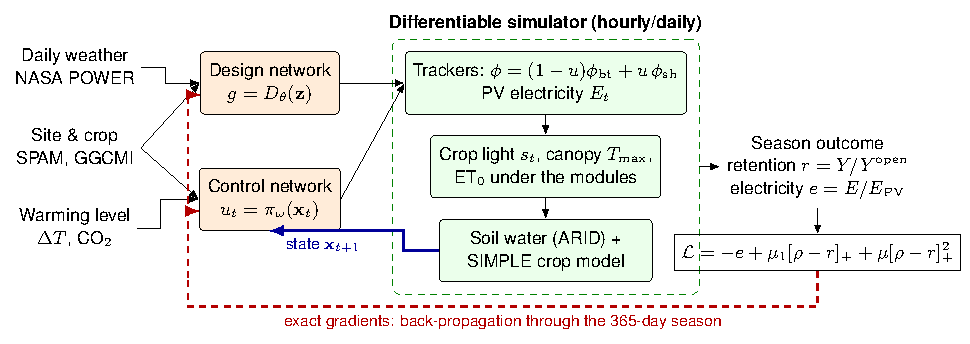
\includegraphics[width=\textwidth]{figures/scheme.pdf}
\caption{SALS. A design network chooses the ground coverage ratio $g$ of single-axis tracker rows from site descriptors, and a control network chooses the daily light-sharing level $u_t$ from the crop, soil and weather state. The differentiable simulator converts these decisions into PV electricity, light and microclimate at the crop, soil water and crop growth. The season's electricity and yield retention enter a penalised objective whose exact gradient is back-propagated through the 365-day season to both networks.}
\label{fig:scheme}
\end{figure}

\begin{figure}[t]
\centering
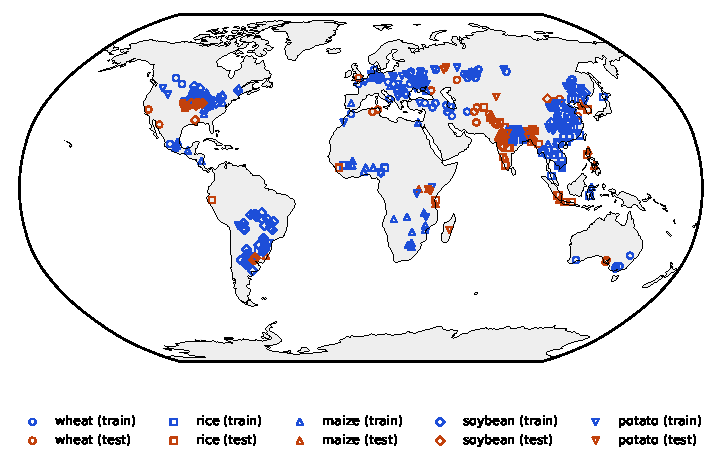
\includegraphics[width=\textwidth]{figures/sites.pdf}
\caption{The 400 crop--site pairs, sampled in proportion to the harvested area of each crop (SPAM 2010). Blue: training sites; orange: geographically held-out test sites (10\textdegree{} blocks).}
\label{fig:map}
\end{figure}

\subsection{Electricity and food on held-out sites and years}\label{sec:main}
Table~\ref{tab:main} and Fig.~\ref{fig:tradeoff} compare the methods on 461 test seasons: 2015--2019 at geographically held-out sites, excluding seasons in which the open-field crop failed ($<0.2$\,t\,ha$^{-1}$). Under the baseline climate, the static agrivoltaic designs that keep 90\% of the yield must use very sparse arrays (GCR $\approx0.10$). They produce 361--377\,MWh\,ha$^{-1}$\,yr$^{-1}$, a quarter of the electricity of a conventional PV plant, and reach an LER of 1.18--1.20. Rotating the trackers to share light with the crop allows denser arrays. The seasonal-sharing and stress rules reach 629 and 707\,MWh\,ha$^{-1}$\,yr$^{-1}$ (LER 1.37 and 1.42), even though their GCR is chosen with knowledge of the test weather. SALS chooses a GCR of 0.34 on average and produces 1019\,MWh\,ha$^{-1}$\,yr$^{-1}$, 72\% of a conventional PV plant, with a mean yield retention of 0.909. Its LER of 1.63 (95\% CI 1.57--1.70) is 0.21 higher than that of the best expert rule and 0.43 higher than that of the static design ($p<10^{-4}$, paired Wilcoxon tests, Table~\ref{tab:stats}). Per-season open-loop optimisation with perfect foresight reached an LER of 1.55. It remained below SALS because optimising 365 daily controls separately for each season is a harder, non-convex problem than learning one policy from thousands of seasons.

\begin{table}[t]
\centering
\caption{Held-out performance (test sites, seasons 2015--2019). GCR: mean ground coverage ratio; $E$: electricity (MWh\,ha$^{-1}$\,yr$^{-1}$); $e$: electricity relative to a conventional PV plant; $r$: mean yield retention; compliance: share of seasons with $r\ge0.9$; LER $=r+e$ with bootstrap 95\% CI over sites. Oracle-GCR baselines choose the GCR with knowledge of the test weather; the open-loop optimisation also knows the daily weather of each test season.}
\label{tab:main}
\small
\begin{tabular}{lcccccc}
\toprule
Method & GCR & $E$ & $e$ & $r$ & Compliance (\%) & LER [95\% CI]\\
\midrule
\multicolumn{7}{l}{\textit{Baseline}}\\
AV static (rule) & 0.10 & 361 & 0.26 & 0.920 & 60.3 & 1.18 [1.16, 1.20]\\
AV static (oracle GCR) & 0.10 & 377 & 0.27 & 0.935 & 85.2 & 1.20 [1.16, 1.25]\\
Seasonal sharing & 0.26 & 629 & 0.45 & 0.921 & 82.2 & 1.37 [1.33, 1.41]\\
Stress rule & 0.23 & 707 & 0.50 & 0.922 & 80.9 & 1.42 [1.37, 1.48]\\
SALS (ours) & 0.34 & \textbf{1019} & 0.72 & 0.909 & 49.5 & 1.63 [1.57, 1.70]\\
Open-loop (foresight) & 0.30 & 916 & 0.65 & 0.901 & 28.6 & 1.55 [1.49, 1.61]\\
\addlinespace
\multicolumn{7}{l}{\textit{+1.5\,\textdegree C}}\\
AV static (rule) & 0.10 & 355 & 0.26 & 0.924 & 66.7 & 1.18 [1.16, 1.20]\\
AV static (oracle GCR) & 0.11 & 385 & 0.28 & 0.931 & 83.5 & 1.21 [1.17, 1.25]\\
Seasonal sharing & 0.28 & 647 & 0.47 & 0.918 & 79.2 & 1.38 [1.34, 1.43]\\
Stress rule & 0.23 & 722 & 0.52 & 0.919 & 77.7 & 1.44 [1.39, 1.49]\\
SALS (ours) & 0.36 & \textbf{1079} & 0.77 & 0.901 & 46.8 & 1.67 [1.61, 1.74]\\
\addlinespace
\multicolumn{7}{l}{\textit{+2\,\textdegree C}}\\
AV static (rule) & 0.10 & 354 & 0.26 & 0.926 & 69.1 & 1.18 [1.16, 1.20]\\
AV static (oracle GCR) & 0.11 & 393 & 0.29 & 0.929 & 83.5 & 1.22 [1.17, 1.26]\\
Seasonal sharing & 0.28 & 659 & 0.48 & 0.917 & 78.9 & 1.39 [1.35, 1.44]\\
Stress rule & 0.23 & 728 & 0.53 & 0.918 & 77.2 & 1.44 [1.39, 1.50]\\
SALS (ours) & 0.37 & \textbf{1106} & 0.79 & 0.898 & 46.3 & 1.69 [1.62, 1.76]\\
\addlinespace
\multicolumn{7}{l}{\textit{+3\,\textdegree C}}\\
AV static (rule) & 0.10 & 353 & 0.26 & 0.933 & 74.2 & 1.19 [1.17, 1.21]\\
AV static (oracle GCR) & 0.12 & 442 & 0.32 & 0.927 & 80.1 & 1.25 [1.20, 1.30]\\
Seasonal sharing & 0.30 & 694 & 0.50 & 0.920 & 78.1 & 1.42 [1.38, 1.47]\\
Stress rule & 0.24 & 762 & 0.55 & 0.919 & 77.7 & 1.47 [1.42, 1.53]\\
SALS (ours) & 0.39 & \textbf{1173} & 0.85 & 0.901 & 45.1 & 1.75 [1.68, 1.82]\\
Open-loop (foresight) & 0.34 & 1028 & 0.74 & 0.901 & 25.8 & 1.65 [1.58, 1.71]\\
\bottomrule
\end{tabular}
\end{table}

\begin{figure}[t]
\centering
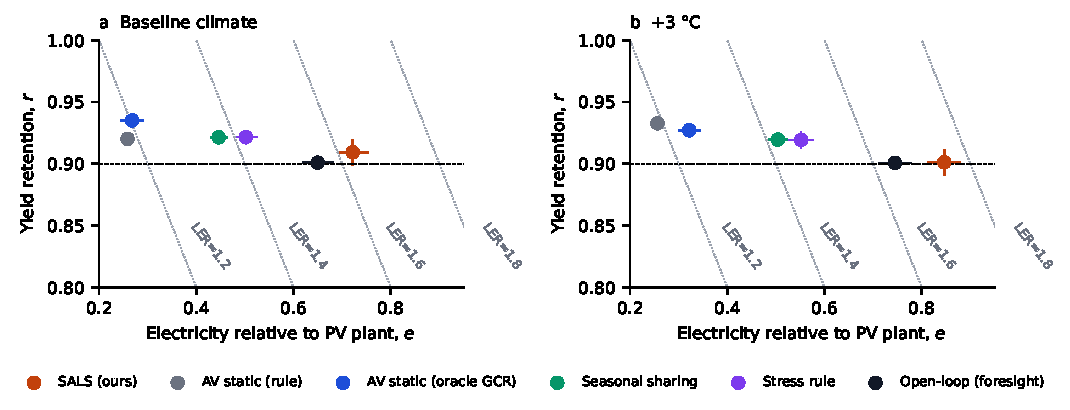
\includegraphics[width=\textwidth]{figures/tradeoff.pdf}
\caption{Electricity--food trade-off on held-out sites and years. Points are means with 95\% confidence intervals; dotted lines are iso-LER lines; the dashed line is the 90\% yield-retention floor.}
\label{fig:tradeoff}
\end{figure}

The gain comes with a trade-off that must be stated clearly. SALS meets the floor \emph{on average}: its mean retention is 0.90--0.91 in all four climates. It meets the floor in only 45--49\% of individual seasons, however, whereas the rule-based baselines meet it in 78--85\% of seasons. The penalty objective (Eq.~\ref{eq:loss}) lets SALS go slightly below the floor in some seasons in exchange for much more electricity. The rules stay above the floor with a margin (mean $r\approx0.92$) and produce 30--65\% less electricity. The floor in Eq.~\eqref{eq:problem} is a per-season constraint; a formulation that guarantees it in a given share of seasons, i.e.\ a chance constraint, would be the natural extension for deployments where regulation is enforced every season (Section~\ref{sec:limits}).

\subsection{What the policy learned}
Fig.~\ref{fig:trajectory} shows the learned control for two of the hottest test seasons under +3\,\textdegree C. For rainfed maize in the Nile Delta, SALS keeps the trackers in energy mode during crop establishment, opens them fully ($u\approx1$) during the canopy-building phase, when intercepted light is most valuable, and returns to energy mode in the second half of the season, when maximum temperatures exceed 40\,\textdegree C and the shade protects the canopy. For irrigated wheat in north-western India, it shares light throughout the cool vegetative phase and shades the crop during the hot grain-filling period before harvest. Over all active crop days of the +3\,\textdegree C test seasons, the mean light-sharing level is 0.33 on days with heat stress and 0.46 on other days. The policy has thus learned to trade light for cooling when heat, not light, limits growth. The design network chooses denser arrays for hotter and drier sites and for maize and soybean (mean GCR 0.42 and 0.39 at present climate) than for wheat and potato (0.32). In these crops, heat and drought limit yield more than light does.

\begin{figure}[t]
\centering
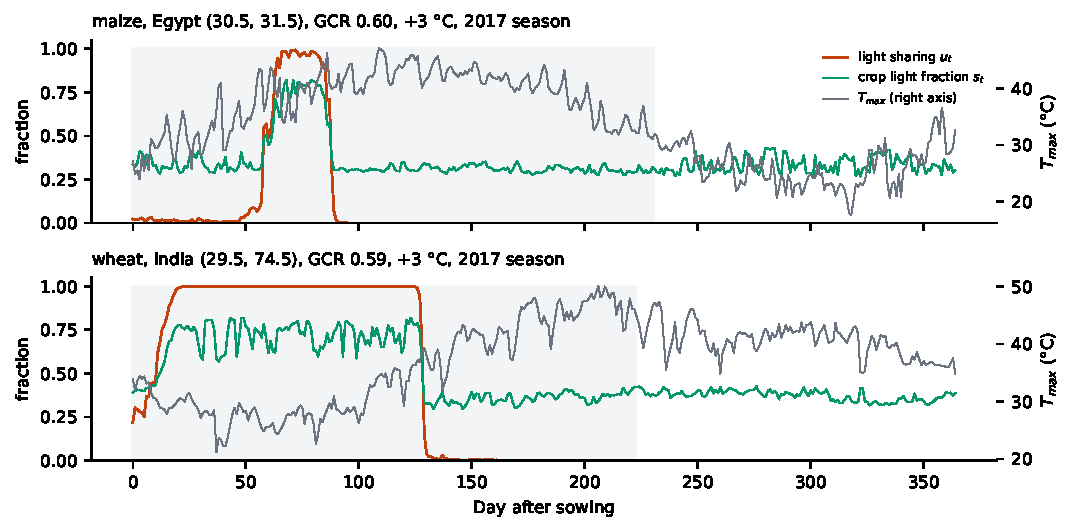
\includegraphics[width=\textwidth]{figures/trajectory.pdf}
\caption{Learned daily control for two hot test seasons under +3\,\textdegree C. Shading marks the cropping season. Orange: light-sharing level $u_t$ chosen by SALS; green: fraction of open-field irradiance reaching the crop; grey: daily maximum temperature (right axis).}
\label{fig:trajectory}
\end{figure}

\subsection{Agrivoltaics under global warming}
Warming changes the balance between light and heat. With the same trained networks, SALS increases its electricity from 1019 to 1079, 1106 and 1173\,MWh\,ha$^{-1}$\,yr$^{-1}$ at +1.5, +2 and +3\,\textdegree C (from 72\% to 85\% of a conventional PV plant) while keeping the mean retention relative to the same-climate open field at 0.90 (Table~\ref{tab:main}). Its LER rises from 1.63 to 1.75, whereas that of the static design stays at about 1.2. Two effects cause this. Warmer seasons are shorter, so the crop occupies the field for fewer days, and heat and drought stress make light less limiting, so more shade can be tolerated or is even beneficial. Across all 400 sites, the SALS system yields more than the open field in 13--14\% of seasons, rising to 31--35\% for maize and 25--28\% for soybean, mostly at hot, rainfed sites (Fig.~\ref{fig:global}b).

Agrivoltaics is not, however, a remedy for the aggregate warming damage. Summed over sites, open-field production of maize and rice falls by 18 and 17\% at +3\,\textdegree C in our simulations, and SALS production by 23 and 26\% relative to the baseline open field, i.e.\ 94 and 90\% of the same-climate open field (Fig.~\ref{fig:warming}). Potato and wheat, which benefit from warmer conditions at cool sites and from CO$_2$ fertilisation in the model, gain in the open field, and SALS keeps 87--89\% of this production. The benefit of SALS under warming is that it maintains the food-security floor while producing more electricity per hectare. It does not reverse the climate impact on yields.

\begin{figure}[t]
\centering
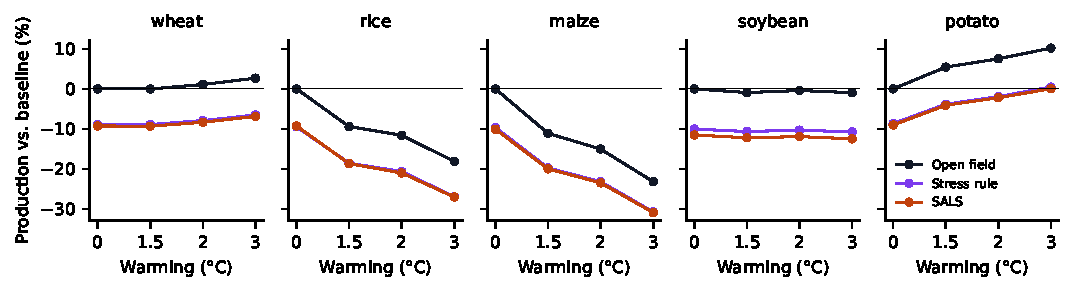
\includegraphics[width=\textwidth]{figures/warming.pdf}
\caption{Production relative to the baseline open field (sum over sites, test years) as a function of warming, for the open field, static agrivoltaics and SALS.}
\label{fig:warming}
\end{figure}

\subsection{Global electricity potential}\label{sec:global}
Fig.~\ref{fig:global} maps the electricity and LER of SALS at all 400 sites. Electricity ranges from a few hundred ha$^{-1}$\,yr$^{-1}$ at high-latitude wheat sites to more than 2000\,MWh\,ha$^{-1}$\,yr$^{-1}$ at sunny, hot maize and soybean sites in South Asia, Africa and the Americas, where the LER exceeds 2. Because the sites were sampled in proportion to harvested area, their mean electricity per hectare can be scaled to the global area of each crop. Deploying SALS agrivoltaics on 5\% of the harvested area of the five crops (33\,Mha) would generate about 31{,}000\,TWh\,yr$^{-1}$ at present climate and 37{,}000\,TWh\,yr$^{-1}$ at +3\,\textdegree C, while retaining on average 93\% of the crop yield on that land. Static agrivoltaic designs with the same yield floor would generate about 11{,}700\,TWh\,yr$^{-1}$. For comparison, global electricity generation was about 30{,}000\,TWh in 2023 \citep{ember2024}. These are technical potentials: they ignore grid integration, storage, land tenure and economic constraints (Section~\ref{sec:limits}). They show, however, that light sharing makes the food-compatible share of cropland large enough to matter for global energy security.

\begin{figure}[t]
\centering
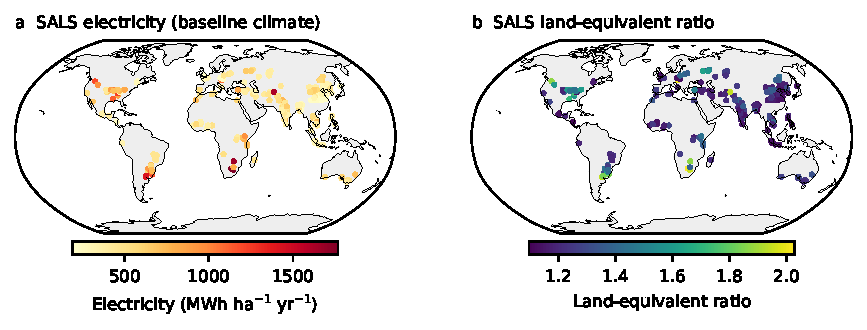
\includegraphics[width=\textwidth]{figures/map.pdf}
\caption{SALS electricity (a) and land-equivalent ratio (b) at the 400 sites (baseline climate, mean of seasons 2015--2019).}
\label{fig:global}
\end{figure}

\subsection{Sensitivity and ablation}\label{sec:sensitivity}
The canopy-cooling coefficient $\kappa$ is the most uncertain microclimate parameter. Evaluated without retraining at $\kappa=0$, 1, 2 and 3\,\textdegree C, the electricity of SALS barely changes (1026--1022\,MWh\,ha$^{-1}$\,yr$^{-1}$ at present climate). Its mean retention changes from 0.871 to 0.931 at present climate and from 0.847 to 0.927 at +3\,\textdegree C. Without any cooling benefit, the policy therefore under-shoots the floor by 3--5 points. The heat-protection effect is thus an important part of the benefit under warming, and field measurements of canopy temperature under trackers are needed to pin it down.

Table~\ref{tab:ablation} reports three ablations. Each variant was trained with the same budget of 200 steps as a reference SALS model and evaluated on the held-out seasons.

\begin{itemize}
\item \emph{Without stress features}: the control network sees only phenology, time, design and crop, with soil water, ARID and the maximum-temperature, irradiance and ET$_0$ forecasts masked. At similar mean retention, this variant produced 28\% less electricity (700 vs 971\,MWh\,ha$^{-1}$\,yr$^{-1}$) and lowered the LER from 1.59 to 1.40 at present climate and from 1.67 to 1.42 at +3\,\textdegree C. A stress-blind policy performs like the expert rules: it learns \emph{when} in the season to share light, but it cannot respond to the heat and drought of a particular season.
\item \emph{Without the design network}: every site uses a GCR of 0.3, close to the mean GCR chosen by SALS, and only the controller is learned. The LER fell to 1.42 and 1.43, and compliance dropped to 31--38\%. The benefit of SALS therefore comes from matching the array density to the site's climate and crop: denser at hot, dry sites where shade is cheap, sparser where light limits growth. The same mean density everywhere does not achieve this.
\item \emph{Trained on the baseline climate only}: the networks were trained on the present climate alone and evaluated in all four climates. They did not learn to exploit the heat-protection value of shade. Their electricity stayed at about 670\,MWh\,ha$^{-1}$\,yr$^{-1}$ and their LER at 1.38--1.40 under all warming levels, whereas the multi-climate model's LER rose from 1.59 to 1.67. This variant was weaker even under the present climate. With a single training seed we cannot separate a regularising effect of the more diverse multi-climate data from optimisation variance, but the result shows that training on projected climates is needed for a policy that remains effective as the climate warms.
\end{itemize}

Training longer (400 instead of 200 steps) added a further 0.04--0.08 to the LER.

\begin{table}[t]
\centering
\caption{Ablation on held-out seasons. $E$: electricity (MWh\,ha$^{-1}$\,yr$^{-1}$); $r$: mean yield retention; C: compliance (\% of seasons with $r\ge0.9$). All ablations were trained for 200 steps and should be compared with SALS (200 steps).}
\label{tab:ablation}
\small
\setlength{\tabcolsep}{4pt}
\begin{tabular}{lcccccccc}
\toprule
 & \multicolumn{4}{c}{Baseline climate} & \multicolumn{4}{c}{+3\,\textdegree C}\\
\cmidrule(lr){2-5}\cmidrule(lr){6-9}
Variant & $E$ & $r$ & C (\%) & LER & $E$ & $r$ & C (\%) & LER\\
\midrule
SALS, full training (400 steps) & 1019 & 0.909 & 49.5 & 1.63 & 1173 & 0.901 & 45.1 & 1.75\\
\midrule
SALS (200 steps) & 971 & 0.897 & 47.3 & 1.59 & 1079 & 0.892 & 43.5 & 1.67\\
w/o stress features & 700 & 0.898 & 33.4 & 1.40 & 706 & 0.906 & 42.7 & 1.42\\
w/o design network (GCR 0.3) & 734 & 0.889 & 31.2 & 1.42 & 719 & 0.900 & 38.1 & 1.43\\
trained on baseline climate only & 668 & 0.904 & 41.4 & 1.38 & 676 & 0.910 & 46.6 & 1.40\\
\bottomrule
\end{tabular}
\end{table}

Finally, we retrained SALS (200 steps) with a softer floor of $\rho=0.8$ and re-evaluated all baselines with the same floor. The baselines' GCR grids and rules were recalibrated for $\rho=0.8$; the static rule then selects GCR 0.15--0.30. Under the present climate, the static design reached an LER of 1.35--1.36, seasonal sharing 1.59 and the stress rule 1.68 (1184\,MWh\,ha$^{-1}$\,yr$^{-1}$). SALS chose much denser arrays (mean GCR 0.55) and produced 1604\,MWh\,ha$^{-1}$\,yr$^{-1}$, 15\% more than a conventional PV plant with GCR 0.4, at a mean retention of 0.815. Its LER was 1.97, rising to 2.03 at +3\,\textdegree C. The ranking of the methods is therefore robust to the choice of the food-security floor. So is the main weakness of SALS: only 38--41\% of its seasons met the 80\% floor, against 74--85\% for the rules. The floor thus steers where SALS operates on the energy--food frontier, but a penalised average does not guarantee it season by season.


\section{Discussion}\label{sec:discussion}

\subsection{What the results establish}
Four findings stand on consistent evidence. First, sharing light with the crop is the main lever on the electricity that tracker-based agrivoltaic arrays can produce under a yield floor. With static trackers the floor limits arrays to about 6\% ground coverage and an LER of 1.07. Any light-sharing control allows about three times the density, and the LER rises to 1.18--1.24 for hand-written rules. Second, the best simple rule follows crop phenology. It shares light across the middle of the season, around flowering and grain filling, and produces electricity at the beginning and the end. It needs only the crop's thermal time, which is observable on the farm, and it is insensitive to forecast errors, whereas the rule that reacts to heat and drought stress is worse in every climate and degrades with forecast error. Third, the qualitative result does not depend on the weakest part of the model. The simulated shade response is conservative against the field trials we could use (Section~\ref{sec:shade}); calibrating it to a meta-analysis or fitting it to the trials raises the allowed density, and the phenology rule stays the best method, with a gain over static arrays of 0.17, 0.19 and 0.30 LER under the conservative, calibrated and field-fitted responses. The absolute gains reported are therefore lower bounds with respect to those trials, not upper bounds, but the trials are few, cover four crops and one or two seasons each, and disagree with the meta-analysis for maize. Fourth, a controller learned through the differentiable simulator is better than the best rule we could write, by 0.03--0.05 in LER and about 10\% in electricity at equal retention, reproducibly over training seeds (range 0.002 in LER), three spatial splits, three canopy-cooling assumptions and four climates, and at 84--86\% of the held-out sites. This gain is small compared with the gap between static and dynamic control.

\subsection{What role does artificial intelligence play?}\label{sec:ai}
The results show where learning matters in this problem and where it does not, and we state this directly because the conclusions would otherwise be overstated. The largest effect, light sharing itself, comes from a physical design choice that a hand-written rule captures. The learned controller refines the timing of that rule and adds 0.03--0.05 LER; a reader who needs a simple, auditable controller can use the phenology rule and obtain about 85\% of the electricity gain of the learned controller over static arrays. The learned policy also has to be initialised from the rule, because training from random weights collapsed to full sharing (Section~\ref{sec:limits}), so we cannot claim that learning discovers the schedule on its own.

Three contributions are specific to the learning approach. First, differentiability is what made the evaluation possible: it allowed us to optimise a policy through whole 365-day seasons for hundreds of crop--site pairs and to screen design variants (density conditioning, floor conditioning, chance-constrained training, forecast noise) at a cost that black-box reinforcement learning \citep{gautron2022} would not allow. Second, the learned policy served as a test of hypotheses about the problem. A network with access to heat, drought and forecast inputs did not use them, and a network without them performed equally well, which supports the conclusion that the benefit comes from phenology and not from stress avoidance, a conclusion that rule design alone could not have reached. Third, one network trained at a single floor remains better than the phenology rule at floors between 0.80 and 0.95, which is a practical advantage for regulations with different floors (+0.033 to +0.037 LER, baseline climate). Conditioning the network on the floor and chance-constrained training gave no further improvement (Section~\ref{sec:extra}). These are, however, modest contributions. A stronger case for learning would need a setting in which the hand-written rule cannot be tuned to the answer, for instance control under uncertainty in the crop response to shade, where one policy has to remain safe across plausible responses, or per-site adaptation from on-farm measurements. We did not test these, and we regard them as the main route by which artificial intelligence could add value beyond what this paper shows.

\subsection{What the results do not establish}
The early hypothesis that stress-aware control, that is, shading the crop on heat and drought days, would be a main source of benefit under warming was not supported. The stress rule performs worse than the phenology rule in every climate, and a learned controller without stress inputs performs as well as one with them. A plausible reason is that in our crop model the yield gain from shading on a hot or dry day is smaller than the loss of light on that day, so stress information does not help. Whether this holds for crop models with more detailed canopy-temperature and heat-stress responses is an open question. Agrivoltaics does not protect staple production against warming in our simulations: light-sharing systems produce about 90\% of the open-field yield in every climate and follow the same decline in maize and rice (Fig.~\ref{fig:warming}).

\subsection{Food security in practice}
Holding the historical mean retention at 90\% does not hold it in each season or at each site. 70\% of SALS seasons meet the floor, the lower tail is slightly heavier than for the rules, and production-weighted retention is below 0.9 for soybean (0.888) and maize (0.898) and in several regions. Chance-constrained design raises season-level compliance to about 92\% at a cost of 0.065 in LER, and the ranking of the controllers is preserved. Whichever formulation is chosen, a per-site regulatory floor would need a region- and crop-specific design step. The upscaled potential (Section~\ref{sec:global}) shows the trade-off in magnitude. The 14\,PWh\,yr$^{-1}$ that 5\% of the staple cropland could supply need about 10\,TWp of modules, several times the present global fleet, and the best sites are rainfed maize and soybean areas where production-weighted retention is lowest.

\subsection{Limitations}\label{sec:limits}
\begin{itemize}
\item \emph{Simulation only.} All results come from a simulator. PV output was benchmarked against PVGIS (29 sites, mean bias $-4.9$\%), but the crop response to shade was only compared with a handful of field trials and one meta-analysis (Section~\ref{sec:shade}). The simulated response is close to proportional, is conservative with respect to the trials (rice, wheat, potato, maize) and does not reproduce the stronger losses of maize and legumes in \citet{laub2022}. The harvest-index sensitivities $h$ are assumptions, and the sensitivity analysis uses rule controllers on a subsample of 22 sites.
\item \emph{Canopy cooling.} The effect of shade on canopy temperature was represented by one coefficient $\kappa$, applied to a heat-stress function that was calibrated on air temperature \citep{siebert2014,webber2018}. The ranking of the controllers is robust to $\kappa$ between 0 and 2\,\textdegree C, but the absolute electricity changes by about $\pm8$\%. Nocturnal warming under modules and rain redistribution are not modelled.
\item \emph{Crop model.} SIMPLE has a fixed harvest index and linear radiation-use efficiency. More detailed models with grain-number formation and canopy energy balance may favour different schedules.
\item \emph{Climate scenarios.} Warming was applied as uniform temperature shifts with fixed precipitation, radiation and relative humidity, and with unchanged cultivars and sowing dates. It is not a bias-adjusted climate projection.
\item \emph{Initialisation and state information.} The network is initialised from the phenology rule, because training from random weights collapsed to full sharing. The gain of SALS is therefore the gain of fine-tuning that rule, and we cannot say whether a better optimiser or a richer policy class would find larger gains. The controller uses the simulated state of the crop and soil (thermal time, canopy interception, soil water) without measurement error, and the forecast errors we tested apply to weather only.
\item \emph{Economics and deployment.} There is no cost, market or grid analysis. The value of midday electricity, curtailment, storage, structural cost and farmer acceptance \citep{trommsdorff2021} will determine the realisable share. The average row pitch at the chosen densities (about 13\,m for 2.2-m modules) leaves room for machinery, but the densest designs (GCR up to 0.5) have a pitch of only 4.4\,m.
\end{itemize}

\section{Conclusions}\label{sec:conclusion}
Light sharing, the daily choice between maximum electricity and letting light through to the crop, is the main lever of tracker-based agrivoltaics under a food-security floor. In a differentiable simulator of trackers, PV output, crop light, microclimate and crop growth, evaluated fairly on 400 crop--site pairs with the array density of each site chosen from its own history, light-sharing rules allowed about three times the module density of static arrays at a mean yield retention of 90\%. They raised the land-equivalent ratio from 1.07 to 1.18--1.24, and a rule that follows crop phenology and needs no weather forecast was the best of them. The simulated shade response is conservative against the field trials we could use, so these gains are lower bounds, and calibrating the response raised them without changing the ranking of methods. A learned controller added a further 0.01--0.05 LER, by following a smooth phenology-dependent schedule that a rule can express; training it on an ensemble of shade responses or giving it a farm-measurable biomass signal added nothing. The part where learning through the differentiable simulator paid off was the calibration of the shade response, which gave an ensemble of plausible responses; designing the array density so that the floor holds in 75\% of them restored the compliance of an oracle design at a cost of 0.02--0.03 LER. The yield floor is met on average but not in every season or region, and the electricity potential of 5\% of staple cropland (about 14\,PWh\,yr$^{-1}$) requires about 10\,TWp of modules. Future work should validate the crop response to shade under trackers with more field data, notably for maize and legumes where the meta-analysis and the trials disagree, extend the crop model to grain-number formation and canopy energy balance, add costs and grid constraints, and pursue controllers that guarantee the food-security floor per site and per season.


\section*{CRediT authorship contribution statement}
\textbf{Quang-Vinh Dang:} Conceptualization, Methodology, Software, Formal analysis, Investigation, Data curation, Visualization, Writing -- original draft, Writing -- review \& editing.

\section*{Declaration of competing interest}
The author has no known competing financial interests or personal relationships that could have appeared to influence the work reported in this paper.

\section*{Data and code availability}
All data used are public: SPAM 2010 v2r0 harvested areas \citep{yu2020}, the GGCMI Phase~3 crop calendar \citep{jagermeyr2021}, NASA POWER daily weather \citep{sparks2018} and the SIMPLE crop parameters \citep{zhao2019}. The code of the simulator, of SALS and of all experiments, together with the site list, is available from the author's public repository (\url{https://github.com/vinhqdang/Artificial-Intelligence-in-Agriculture}).

\section*{Funding}
This research did not receive any specific grant from funding agencies in the public, commercial, or not-for-profit sectors.

\appendix
\section{Statistical comparison}\label{app:stats}
\begin{table}[h]
\centering
\caption{Paired comparison of SALS with each baseline on the 92 held-out sites of the main split (unit of analysis: site mean over test seasons). $\Delta$LER: mean difference (SALS minus baseline) with cluster-bootstrap 95\% CI; $p$: two-sided Wilcoxon signed-rank test; \% better: share of sites where SALS has the higher LER; $\Delta r$: difference in mean yield retention with its Wilcoxon $p$-value.}
\label{tab:stats}
\scriptsize
\setlength{\tabcolsep}{3pt}
\begin{tabular}{llccccccc}
\toprule
Climate & Baseline & $\Delta$LER [95\% CI] & $p$ & \% better & $\Delta r$ & $p$ & Sites\\
\midrule
Baseline & AV static & +0.205 [+0.176, +0.236] & $<10^{-4}$ & 100 & -0.011 & $<10^{-4}$ & 92\\
Baseline & Seasonal sharing & +0.088 [+0.068, +0.109] & $<10^{-4}$ & 97 & +0.001 & 0.922 & 92\\
Baseline & Phenology rule & +0.038 [+0.025, +0.053] & $<10^{-4}$ & 84 & +0.001 & 0.723 & 92\\
Baseline & Stress rule & +0.096 [+0.071, +0.124] & $<10^{-4}$ & 93 & -0.002 & 0.055 & 92\\
+1.5\,\textdegree C & AV static & +0.208 [+0.180, +0.237] & $<10^{-4}$ & 100 & -0.010 & $<10^{-4}$ & 92\\
+1.5\,\textdegree C & Seasonal sharing & +0.095 [+0.077, +0.114] & $<10^{-4}$ & 98 & +0.001 & 0.812 & 92\\
+1.5\,\textdegree C & Phenology rule & +0.033 [+0.022, +0.045] & $<10^{-4}$ & 86 & +0.002 & 0.855 & 92\\
+1.5\,\textdegree C & Stress rule & +0.108 [+0.083, +0.134] & $<10^{-4}$ & 98 & -0.001 & 0.041 & 92\\
+2\,\textdegree C & AV static & +0.209 [+0.181, +0.238] & $<10^{-4}$ & 100 & -0.010 & $<10^{-4}$ & 92\\
+2\,\textdegree C & Seasonal sharing & +0.097 [+0.079, +0.115] & $<10^{-4}$ & 97 & +0.001 & 0.876 & 92\\
+2\,\textdegree C & Phenology rule & +0.032 [+0.022, +0.044] & $<10^{-4}$ & 85 & +0.002 & 0.496 & 92\\
+2\,\textdegree C & Stress rule & +0.115 [+0.089, +0.142] & $<10^{-4}$ & 98 & -0.003 & 0.016 & 92\\
+3\,\textdegree C & AV static & +0.219 [+0.190, +0.250] & $<10^{-4}$ & 100 & -0.009 & $<10^{-4}$ & 92\\
+3\,\textdegree C & Seasonal sharing & +0.108 [+0.089, +0.129] & $<10^{-4}$ & 96 & +0.001 & 0.935 & 92\\
+3\,\textdegree C & Phenology rule & +0.034 [+0.022, +0.046] & $<10^{-4}$ & 86 & +0.002 & 0.330 & 92\\
+3\,\textdegree C & Stress rule & +0.131 [+0.102, +0.162] & $<10^{-4}$ & 98 & -0.002 & 0.142 & 92\\
\bottomrule
\end{tabular}
\end{table}


\bibliographystyle{elsarticle-harv}
\bibliography{references}

\end{document}
